\documentclass{article}\usepackage[]{graphicx}\usepackage[]{color}
%% maxwidth is the original width if it is less than linewidth
%% otherwise use linewidth (to make sure the graphics do not exceed the margin)
\makeatletter
\def\maxwidth{ %
  \ifdim\Gin@nat@width>\linewidth
    \linewidth
  \else
    \Gin@nat@width
  \fi
}
\makeatother

\definecolor{fgcolor}{rgb}{0.345, 0.345, 0.345}
\newcommand{\hlnum}[1]{\textcolor[rgb]{0.686,0.059,0.569}{#1}}%
\newcommand{\hlstr}[1]{\textcolor[rgb]{0.192,0.494,0.8}{#1}}%
\newcommand{\hlcom}[1]{\textcolor[rgb]{0.678,0.584,0.686}{\textit{#1}}}%
\newcommand{\hlopt}[1]{\textcolor[rgb]{0,0,0}{#1}}%
\newcommand{\hlstd}[1]{\textcolor[rgb]{0.345,0.345,0.345}{#1}}%
\newcommand{\hlkwa}[1]{\textcolor[rgb]{0.161,0.373,0.58}{\textbf{#1}}}%
\newcommand{\hlkwb}[1]{\textcolor[rgb]{0.69,0.353,0.396}{#1}}%
\newcommand{\hlkwc}[1]{\textcolor[rgb]{0.333,0.667,0.333}{#1}}%
\newcommand{\hlkwd}[1]{\textcolor[rgb]{0.737,0.353,0.396}{\textbf{#1}}}%

\usepackage{framed}
\makeatletter
\newenvironment{kframe}{%
 \def\at@end@of@kframe{}%
 \ifinner\ifhmode%
  \def\at@end@of@kframe{\end{minipage}}%
  \begin{minipage}{\columnwidth}%
 \fi\fi%
 \def\FrameCommand##1{\hskip\@totalleftmargin \hskip-\fboxsep
 \colorbox{shadecolor}{##1}\hskip-\fboxsep
     % There is no \\@totalrightmargin, so:
     \hskip-\linewidth \hskip-\@totalleftmargin \hskip\columnwidth}%
 \MakeFramed {\advance\hsize-\width
   \@totalleftmargin\z@ \linewidth\hsize
   \@setminipage}}%
 {\par\unskip\endMakeFramed%
 \at@end@of@kframe}
\makeatother

\definecolor{shadecolor}{rgb}{.97, .97, .97}
\definecolor{messagecolor}{rgb}{0, 0, 0}
\definecolor{warningcolor}{rgb}{1, 0, 1}
\definecolor{errorcolor}{rgb}{1, 0, 0}
\newenvironment{knitrout}{}{} % an empty environment to be redefined in TeX

\usepackage{alltt}
\usepackage[english]{babel}
\IfFileExists{upquote.sty}{\usepackage{upquote}}{}
\begin{document}
\title{Marsh Elevation Monitoring\\
The Nature Conservancy, \\
Long Island NY}
\author{Nicole Maher \& Adam Starke}
\maketitle\thispagestyle{empty}





\section{Intro}
The following is a quick compilation of the trends that have been measured at sites being monitored by TNC across Long Island. Note that data is not complete and still needs to be verified fully. The rate of the overall change in elevation is calcuated by finding the average change in each of 9 pins from the start of the monitoring period to the present. More directly, a linear regression is fit to the height of the pins through time. These lines are then averaged across stations for each site. 

Project area:
\begin{kframe}


{\ttfamily\noindent\bfseries\color{errorcolor}{\#\# Error: cannot open URL 'http://b.tile.cloudmade.com/c669db620b804a3a90fbe4193c4c6ec8/125286@2x/256/10/301/383.png'}}

{\ttfamily\noindent\bfseries\color{errorcolor}{\#\# Error: object 'Site.blankmap' not found}}\end{kframe}

Tables:
% latex table generated in R 3.0.2 by xtable 1.7-3 package
% Wed May 14 16:49:19 2014
\begin{table}[ht]
\centering
\begin{tabular}{rlllrrrrrr}
  \hline
 & Site\_Name & Stratafication & SET\_Type & Sample N & Mean\_elevation\_change & SE\_ofmeanrate & Mean\_Accretion\_Rate & SE of mean Accrretion mm/yr & SubSurface\_change \\ 
  \hline
1 & Accobonac Harbor & Low Marsh & Rod SET &  14 & 3.14 & 0.29 & 2.56 & 0.26 & 0.58 \\ 
  2 & Bass Creek & Low Marsh & Rod SET &  15 & 4.83 & 0.19 & 5.30 & 0.26 & -0.47 \\ 
  3 & Bass Creek & Low Marsh & Shallow SET &   2 &  &  & 5.30 & 0.26 &  \\ 
  4 & Cedar Beach & Low Marsh & Rod SET &   9 & 3.79 & 1.70 & 8.84 & 0.87 & -5.05 \\ 
  5 & Hubbard Creek & Low Marsh & Rod SET &  13 & 3.18 & 0.37 & 3.91 & 0.81 & -0.73 \\ 
  6 & Indian Island & High Marsh & Rod SET &   9 & 2.58 & 0.19 & 2.60 & 0.66 & -0.02 \\ 
  7 & Indian Island & Low Marsh & Rod SET &   9 & 3.68 & 0.14 & 5.05 & 0.09 & -1.37 \\ 
  8 & Lawrence Marsh & Low Marsh & Rod SET &   3 & -0.78 & 0.48 & 2.58 & 1.43 & -3.36 \\ 
  9 & Lawrence Marsh & Low Marsh & Shallow SET &   3 & 0.95 & 1.32 & 2.58 & 1.43 & -1.63 \\ 
  10 & Mashomack Point & Low Marsh & Rod SET &   9 & 5.01 & 0.53 & 7.66 & 0.30 & -2.65 \\ 
  11 & Mashomack Point & Low Marsh & Shallow SET &   2 &  &  & 7.66 & 0.30 &  \\ 
  12 & North Greensedge - West Hempstead & Low Marsh & Rod SET &   3 & 1.05 & 1.32 & 4.20 & 0.40 & -3.15 \\ 
  13 & North Greensedge - West Hempstead & Low Marsh & Shallow SET &   3 & 3.17 & 1.00 & 4.20 & 0.40 & -1.03 \\ 
  14 & Pine Neck & High Marsh & Rod SET &   8 & 4.73 & 0.13 & 4.07 & 0.23 & 0.66 \\ 
  15 & Pine Neck & High Marsh & Shallow SET &   2 &  &  & 4.07 & 0.23 &  \\ 
  16 & Pine Neck & Low Marsh & Rod SET &   8 & 6.73 & 0.73 & 8.13 & 0.42 & -1.40 \\ 
  17 & Pine Neck & Low Marsh & Shallow SET &   2 &  &  & 8.13 & 0.42 &  \\ 
   \hline
\end{tabular}
\caption{SET-MH monitoring sites across Long Island} 
\end{table}




\section{Visuals}
What follows is a quick visual of the changes that have been measured along the marsh surfaces. The rate of the overall change in elevation is calcuated by finding the average change in each of 9 pins from the start of the monitoring period to the present. More directly, a linear regression is fit to the height of the pins through time. These lines are then averaged across stations for each site. 



{\centering 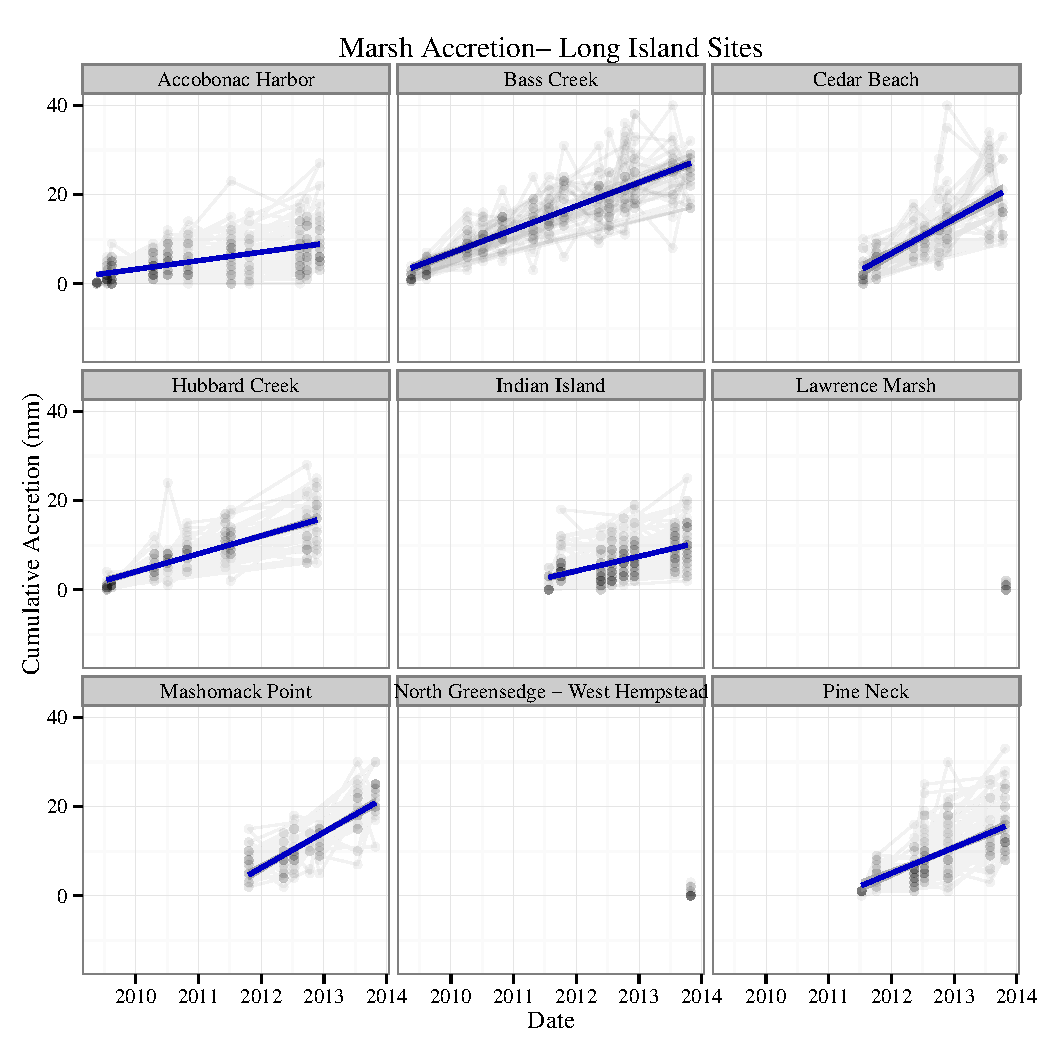
\includegraphics[width=\maxwidth]{figure/SA_Plots} 

}







{\centering 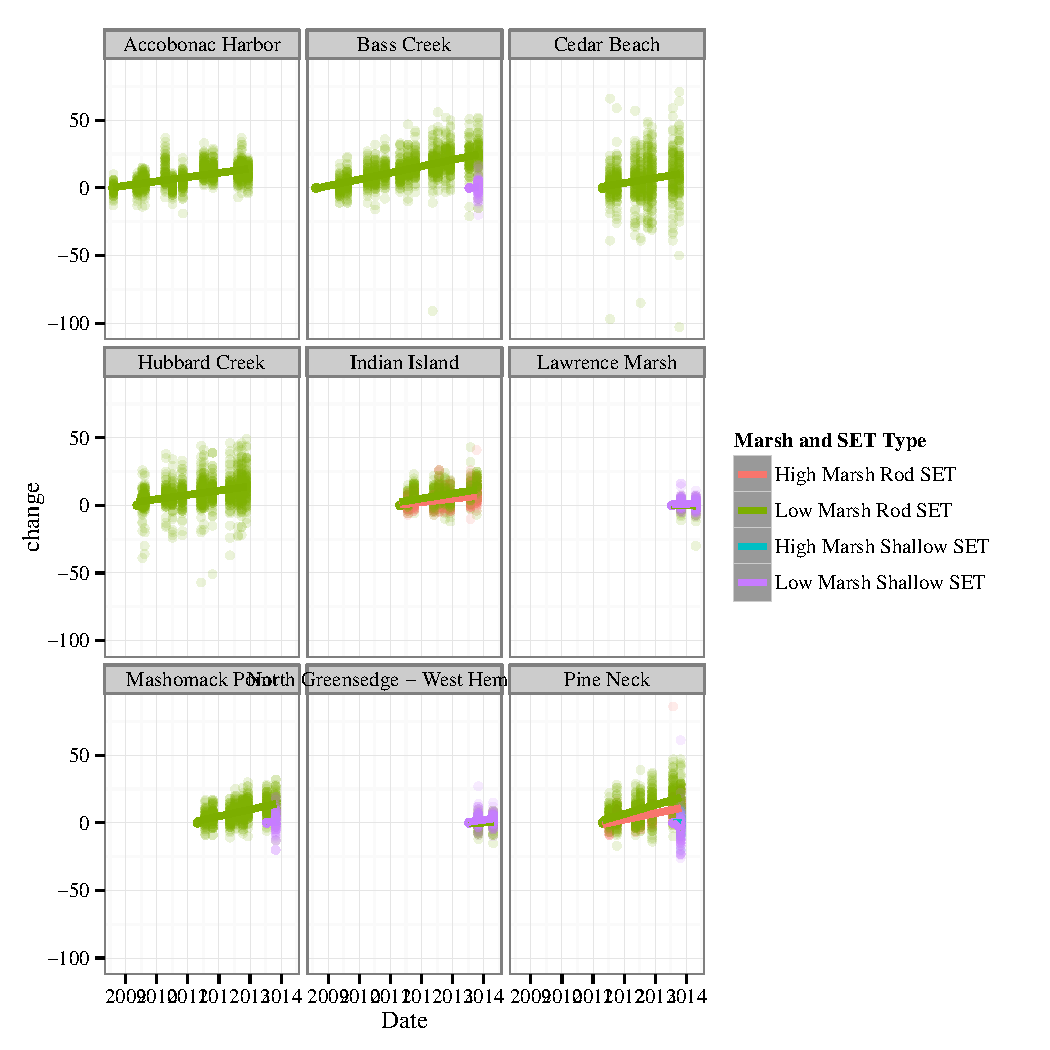
\includegraphics[width=\maxwidth]{figure/Plot_multiLMs} 

}







\end{document}
